\subsection{Simulation}\label{chSMS_ID.sec.SO3_AID_Sim}

This Section describes the performance of the proposed \ac{AID}
algorithm in numerical simulation.  The numerical results presented
herein used a fourth order Runge-Kutta numerical solution to simulate
both the \ac{AID} algorithm, (\ref{chSMS_ID.eq.SO3_AID_estimator})
and (\ref{chSMS_ID.eq.SO3_AID_identifier}), and the plant,
(\ref{chModels.eq.SO3plant}).  Since the \ac{AID} algorithm assumed
access to both $\omega(t)$ and $\tau(t)$, without loss of generality we
choose $\hat{\omega}(t_0)=\omega(t_0)$. The input torque $\tau(t)$ was
generated as a sum of sines and cosines, each with different
frequencies and amplitudes.  In each trial the plant's inertia tensor,
$I$, was chosen and the inertia tensor estimate was initialized to the
identity matrix, i.e. $\hat{I}(t_0)=\mathbb{I}$.


\subsubsection{Convergence of State and Parameter Estimates}

To test the differences in identification performance we explored the
effects of factors including initial parameter error, input torque
richness, and feedback gain.  Figure \ref{chSMS_ID.fig.SO3_AID_basic} is
representative of simulated performance in the majority of cases.
This representative simulation study used a
feedback gain $a=1$; an input torque of
%
\begin{equation}
\tau(t)=\left[ \begin{array}{ccc}-2\cos(2t)& -2\sin(t)
    &2cos(t)\end{array}\right]^{T};
\end{equation}
%
an inertia tensor of $I=1.5\mathbb{I}$; and an estimate of
$\hat{I}(t_0)=\mathbb{I}$ (this was the initial inertia tensor for
every simulation study in this Section).  This Figure explicitly shows
state and parameter convergence of the angular velocity and inertia
tensor eigenvalue estimates.  The eigenvalues of the \ac{SPD} inertia
tensors are plotted to show parameter convergence.

\begin{center}
\begin{figure}[htbp]
  \begin{center}
    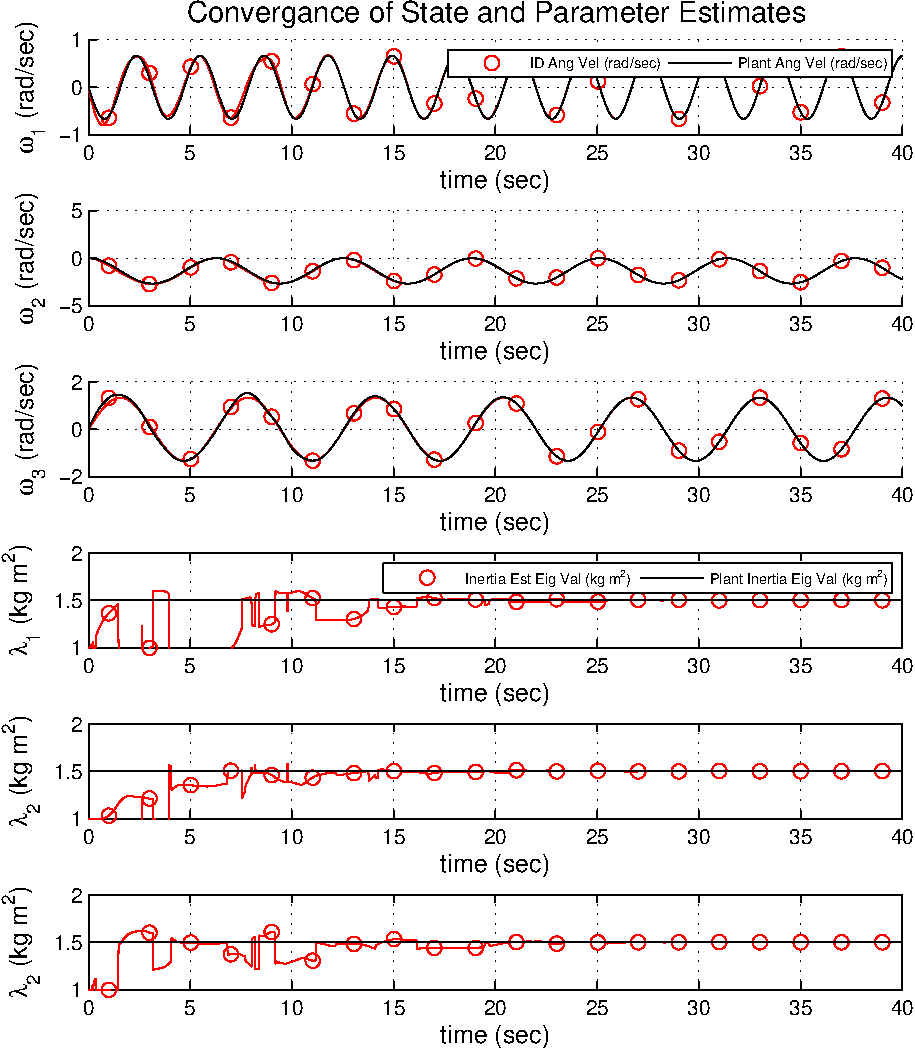
\includegraphics[width=150mm]{./chSMS_ID/images/SO3AID_stateParamConv}
  \end{center}
  \caption{ Data showing state and parameter convergence during a
    representative simulation study.  Estimated values are highlighted
    with circles.  The top three plots show the estimated angular
    velocity's convergence to the true plant angular velocity in each
    \ac{DOF}.  The bottom three plots show the eigenvalues of the
    estimated inertia tensor converging the true inertia tensor
    eigenvalues.}
  \label{chSMS_ID.fig.SO3_AID_basic}
\end{figure}
\end{center}


\subsubsection{Effect of Scalar feedback Gain Parameter $a$}

Figure \ref{chSMS_ID.fig.SO3_AID_gains} shows how \ac{AID} algorithm performance
varies with changes of the scalar gain $a$.  In the case that $a$ is
large, the angular velocity error remains small for all time, and  the
small angular velocity error limits the ability of this error signal
to drive parameter adaptation as seen in
(\ref{chSMS_ID.eq.SO3_AID_identifier}).  For the case of very small
values of $a$, the parameter convergence is slow.  In the limiting
case of $a=0$ the identifier is stable, but not asymptotically stable.

\begin{center}
\begin{figure}[htbp]
  \begin{center}
    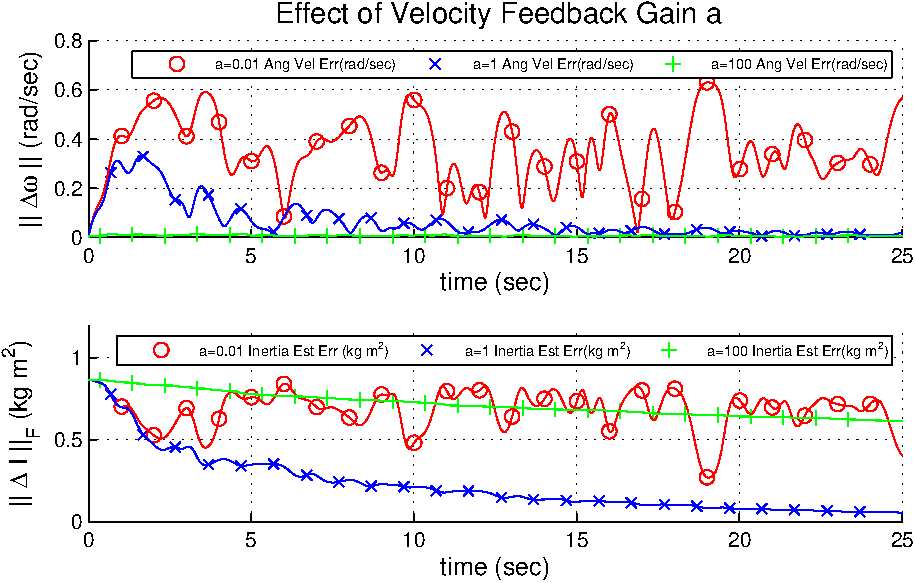
\includegraphics[width=150mm]{./chSMS_ID/images/gainFig01}
  \end{center}
  \caption{The effect of the feedback gain, $a$, on angular velocity and
    parameter convergence.  The upper graph plots the norm of the body
    angular velocity error versus time.  The lower graph plots the
    Frobenius norm of the inertia tensor error versus time.  The cases
    of \ac{AID} for $a=0.01$, $a=1.0$, and $a=100$ are
    shown.  Parameter convergence deteriorates for very large and very
    small gains.  }  \label{chSMS_ID.fig.SO3_AID_gains}
\end{figure}
\end{center}

\subsubsection{Effect of Input $\tau(t)$ Richness}

Figure \ref{chSMS_ID.fig.SO3_AID_perExcit} demonstrates the well know
fact that exact parameter identification requires a sufficiently rich
input torque signal.  For these simulations we employed the following
values for the identification algorithm: $a=1$, $I=1.5\mathbb{I}$,
$\hat{I}(t_0)=\mathbb{I}$, and either
$\tau(t)=\left[\begin{array}{ccc}-2\cos(2t)& -2\sin(t)&
    2\cos(t)\end{array}\right]^{T}$ or
$\tau(t)=\left[\begin{array}{ccc}0& -2\sin(t)&
    0\end{array}\right]^{T}$.  In both cases the estimated angular
velocity converged to the true angular velocity. For the case of the
richer input signal, the inertia tensor estimate converged to the
actual plant inertia tensor value.  
%
For the case of the simple input signal, however, the inertia tensor
estimate converged to a value different from the plant's inertia
tensor value.
%
Note that the inertia tensor estimate still converged to a value that
results in identical input-output behavior of the {\it estimated
  plant} and actual plant for this simple input signal (where an {\it
  estimated plant} is a second-order rotational plant of the form
(\ref{chModels.eq.SO3plant}) with its inertia tensor equal to an
inertia tensor estimate).


 \begin{center}
 \begin{figure}[htbp]
   \begin{center}
     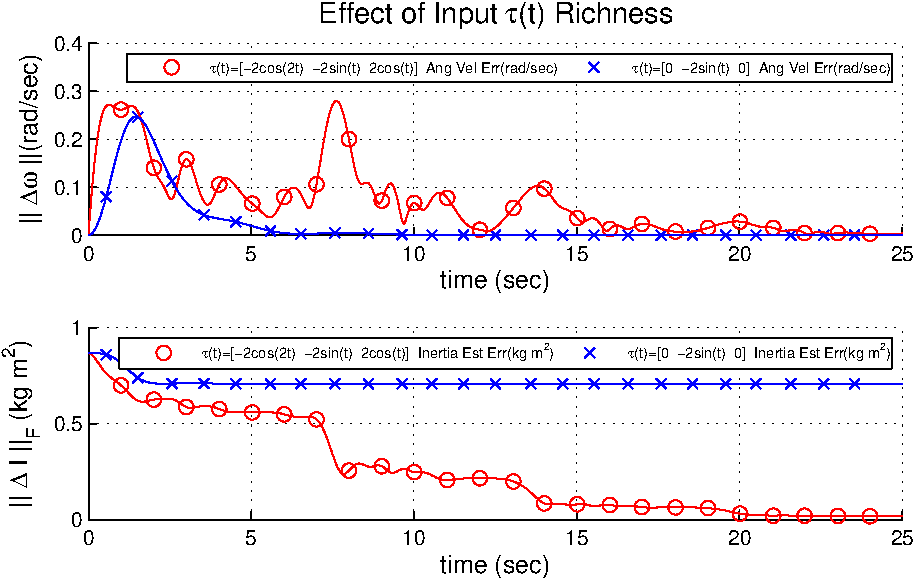
\includegraphics[width=150mm]{./chSMS_ID/images/perExcit01}
   \end{center}
   \caption{ Two plots showing that parameter convergence requires a
     sufficiently rich input signal.  The upper graph plots the norm
     of the body angular velocity error versus time for two inputs
     $\tau(t)$.  The lower graph plots the Frobenius norm of the inertia
     tensor error versus time for both cases.  The angular velocity
     estimate converges in either case. $\tau(t)=[0\quad -2\sin(t)\quad 0]$ is not
     rich enough to force parameter convergence for this initial
     condition, whereas parameter convergence occurs for input torque
     $\tau(t)=[-2\cos(2t)\quad -2\sin(t)\quad 2\cos(t)]$.  }
   \label{chSMS_ID.fig.SO3_AID_perExcit}
 \end{figure}
 \end{center}

\subsubsection{Effect of $\hat{I}(t_0)$}


This Section examines the effect of initial parameter estimate error,
$\Delta I(t_0)$, on parameter convergence. Figure
\ref{chSMS_ID.fig.SO3_AID_smallRange} shows parameter convergence for
30 simulated initial conditions. In all cases
$\hat{I}(t_0)=\mathbb{I}$ and $a=1$. In each case $\tau(t)$ was generated
from sums of sinusoids of different frequencies with randomly
generated amplitudes.  Three sets of ten inertia tensors were used.
Every inertia tensor was randomly generated such that it was a
non-diagonal \ac{SPD} matrix with the eigenvalues greater than
0.5. Within each set the Frobenius norm of $\|\Delta I(t_0)\|_F$ was
either 0.15, 0.5, or 1. Figure \ref{chSMS_ID.fig.SO3_AID_smallRange}
plots parameter convergence of the \ac{AID} algorithm to every
inertia tensor in each of the three sets. For sets one and two, with
$\|\Delta I(t_0)\|_F=0.15$ and $\|\Delta I(t_0)\|_F=0.5$, all
conditions of Theorem \ref{chSMS_ID.theo.SO3_AID} were met. For set
three, often $\|\Delta I(t_0)\|_F>\lambda_3$ and thus the conditions
of Theorem \ref{chSMS_ID.theo.SO3_AID} were not met.  Despite this,
every inertia tensor estimate converged to the true inertia tensor for
each randomly generated initial condition. This convergence
corroborates our analytic result and indicates that the condition
requiring $\|\Delta I(t_0)\|_F<\lambda_3$ from Theorem
\ref{chSMS_ID.theo.SO3_AID} is sufficient but not necessary for
asymptotic convergence.


\begin{center}
\begin{figure}[htbp]
  \begin{center}
    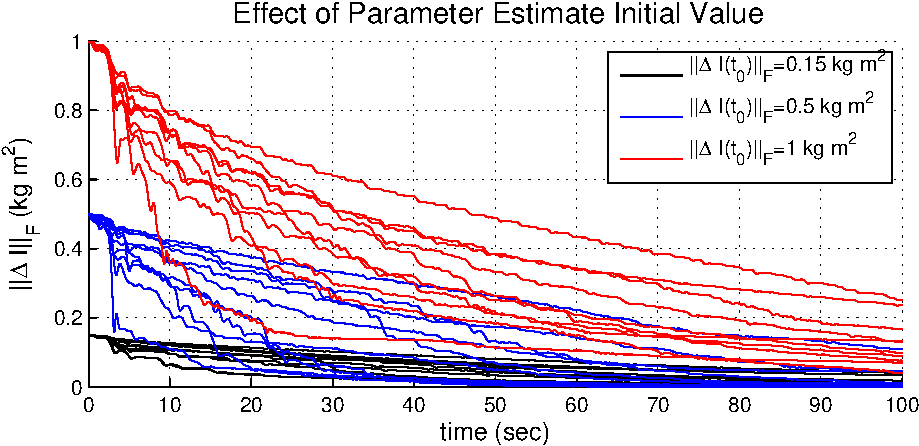
\includegraphics[width=150mm]{./chSMS_ID/images/inertiaEstimateInitErr}
  \end{center}
  \caption{ Three sets of ten simulations showing parameter
    convergence.  The Frobenius norm of the inertia tensor error is
    plotted versus time. Each of the simulations used a randomly
    selected inertia tensor for the system, but within each set the
    Frobenius norm of the initial inertia error was a constant value
    for the entire set, either 0.15, 0.5, or 1.}
  \label{chSMS_ID.fig.SO3_AID_smallRange}
\end{figure}
\end{center}


%\begin{center}
%\begin{figure}[htbp]
%  \begin{center}
%    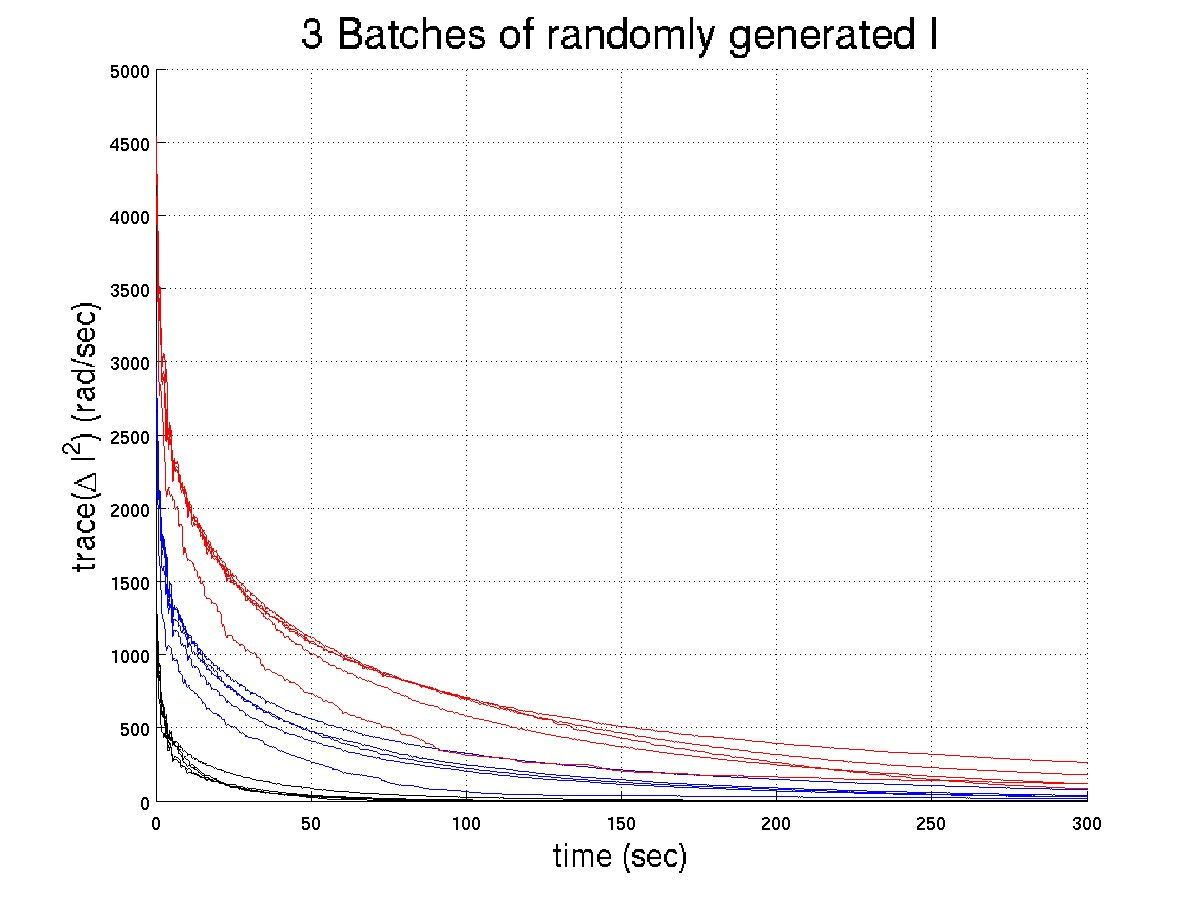
\includegraphics[width=90mm]{./images/largeRangeFig}
%  \end{center}
%  \caption{ 3 sets of 5 simulations of parameter convergence, with
%    each set having a random initialization but a set error between I
%    and $\hat{I}(t_0)$.  Note that for all three set of 5 the
%    parameter error is many orders of magnitude larger than errors
%    which would meet the conditions set forth in Theorem \ref{SO3_ID}.}
%  \label{fig:largeRange}
%\end{figure}
%\end{center}

%One of the most limiting requirements of Theorem \ref{SO3_ID} is the
%requirement for $\hat{I}(t_0)$ to start so close in the neighborhood
%of $I$.  Since both $\hat{I}(t)$ and $\hat{I}(t)^{-1}$ appear in the
%parameter update law, the neighborhood requirement stated in Theorem
%\ref{SO3_ID} was chosen such that Lyapunov Stability would make
%reaching a singularity impossible.  In practice, especially if the
%eigenvalues of the true Moment of Inertia are much larger than the
%Moment of Inertia eigenvalues which the identification algorithm is
%initialized at, our experience is that the neighborhood requirement
%placed on $\hat{I}(t_0)$ is very conservative.   

